\documentclass[aspectratio=169]{../latex_main/tntbeamer}  % you can pass all options of the beamer class, e.g., 'handout' or 'aspectratio=43'
\usepackage{dsfont}
\usepackage{bm}
\usepackage[english]{babel}
\usepackage[T1]{fontenc}
%\usepackage[utf8]{inputenc}
\usepackage{graphicx}
\graphicspath{ {./figures/} }
\usepackage{algorithm}
\usepackage[ruled,vlined,algo2e,linesnumbered]{algorithm2e}
\usepackage{hyperref}
\usepackage{booktabs}
\usepackage{mathtools}

\usepackage{amsmath,amssymb}

\DeclareMathOperator*{\argmax}{arg\,max}
\DeclareMathOperator*{\argmin}{arg\,min}

\usepackage{amsbsy}
\newcommand{\vect}[1]{\bm{#1}}
%\newcommand{\vect}[1]{\boldsymbol{#1}}

\usepackage{pgfplots}
\pgfplotsset{compat=1.16}
\usepackage{tikz}
\usetikzlibrary{trees} 
\usetikzlibrary{shapes.geometric}
\usetikzlibrary{positioning,shapes,shadows,arrows,calc,mindmap}
\usetikzlibrary{positioning,fadings,through}
\usetikzlibrary{decorations.pathreplacing}
\usetikzlibrary{intersections}
\pgfdeclarelayer{background}
\pgfdeclarelayer{foreground}
\pgfsetlayers{background,main,foreground}
\tikzstyle{activity}=[rectangle, draw=black, rounded corners, text centered, text width=8em]
\tikzstyle{data}=[rectangle, draw=black, text centered, text width=8em]
\tikzstyle{myarrow}=[->, thick, draw=black]

% Define the layers to draw the diagram
\pgfdeclarelayer{background}
\pgfdeclarelayer{foreground}
\pgfsetlayers{background,main,foreground}

% Requires XeLaTeX or LuaLaTeX
%\usepackage{unicode-math}

\usepackage{fontspec}
%\setsansfont{Arial}
\setsansfont{RotisSansSerifStd}[ 
Path=../latex_main/fonts/,
Extension = .otf,
UprightFont = *-Regular,  % or *-Light
BoldFont = *-ExtraBold,  % or *-Bold
ItalicFont = *-Italic
]
\setmonofont{Cascadia Mono}[
Scale=0.8
]

% scale factor adapted; mathrm font added (Benjamin Spitschan @TNT, 2021-06-01)
%\setmathfont[Scale=1.05]{Libertinus Math}
%\setmathrm[Scale=1.05]{Libertinus Math}

% other available math fonts are (not exhaustive)
% Latin Modern Math
% XITS Math
% Libertinus Math
% Asana Math
% Fira Math
% TeX Gyre Pagella Math
% TeX Gyre Bonum Math
% TeX Gyre Schola Math
% TeX Gyre Termes Math

% Literature References
\newcommand{\lit}[2]{\href{#2}{\footnotesize\color{black!60}[#1]}}

%%% Beamer Customization
%----------------------------------------------------------------------
% (Don't) Show sections in frame header. Options: 'sections', 'sections light', empty
\setbeamertemplate{headline}{empty}

% Add header logo for normal frames
\setheaderimage{
	% 
\includegraphics[height=\logoheight]{figures/TNT_darkv4.pdf}
	
\includegraphics[height=\logoheight]{../latex_main/figures/luh_logo_rgb_0_80_155.pdf}
	% 
\includegraphics[height=\logoheight]{figures/logo_tntluh.pdf}
}

% Header logo for title page
\settitleheaderimage{
	% 
\includegraphics[height=\logoheight]{figures/TNT_darkv4.pdf}
	
\includegraphics[height=\logoheight]{../latex_main/figures/luh_logo_rgb_0_80_155.pdf}
	% 
\includegraphics[height=\logoheight]{figures/logo_tntluh.pdf}
}

% Title page: tntdefault 
\setbeamertemplate{title page}[tntdefault]  % or luhstyle
% Add optional title image here
%\addtitlepageimagedefault{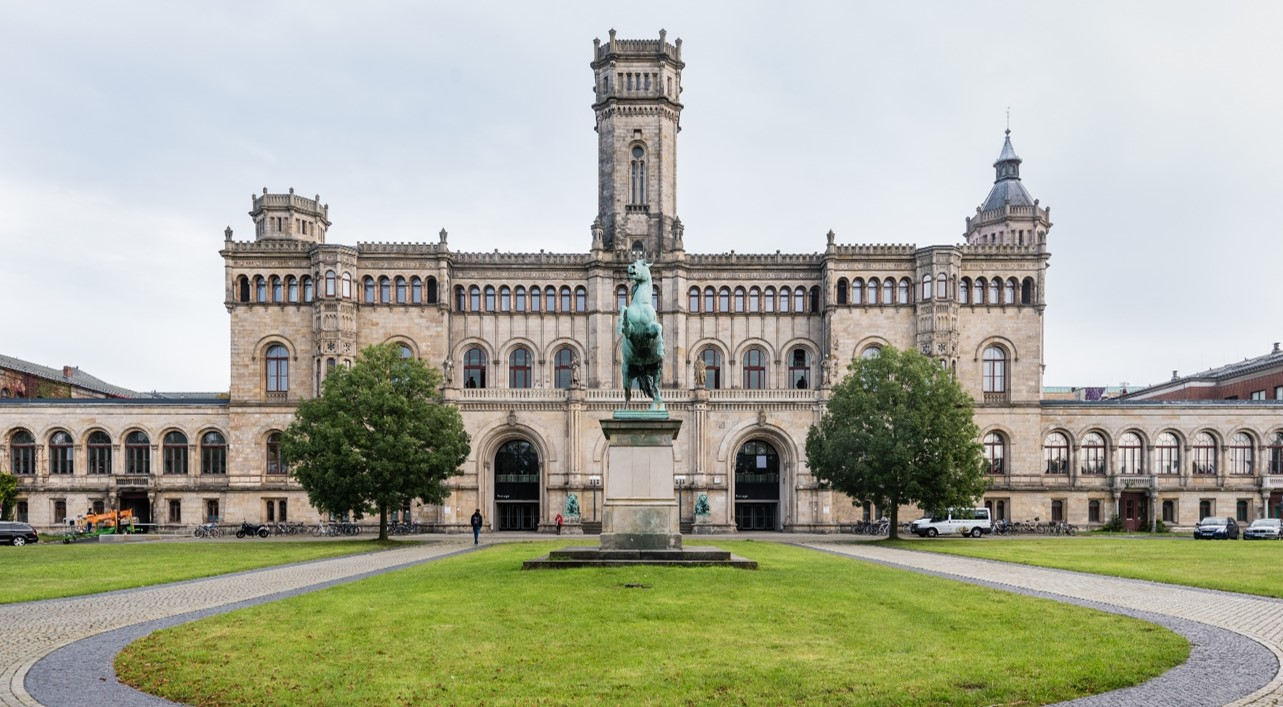
\includegraphics[width=0.65\textwidth]{figures/luh_default_presentation_title_image.jpg}}

% Title page: luhstyle
% \setbeamertemplate{title page}[luhstyle]
% % Add optional title image here
% \addtitlepageimage{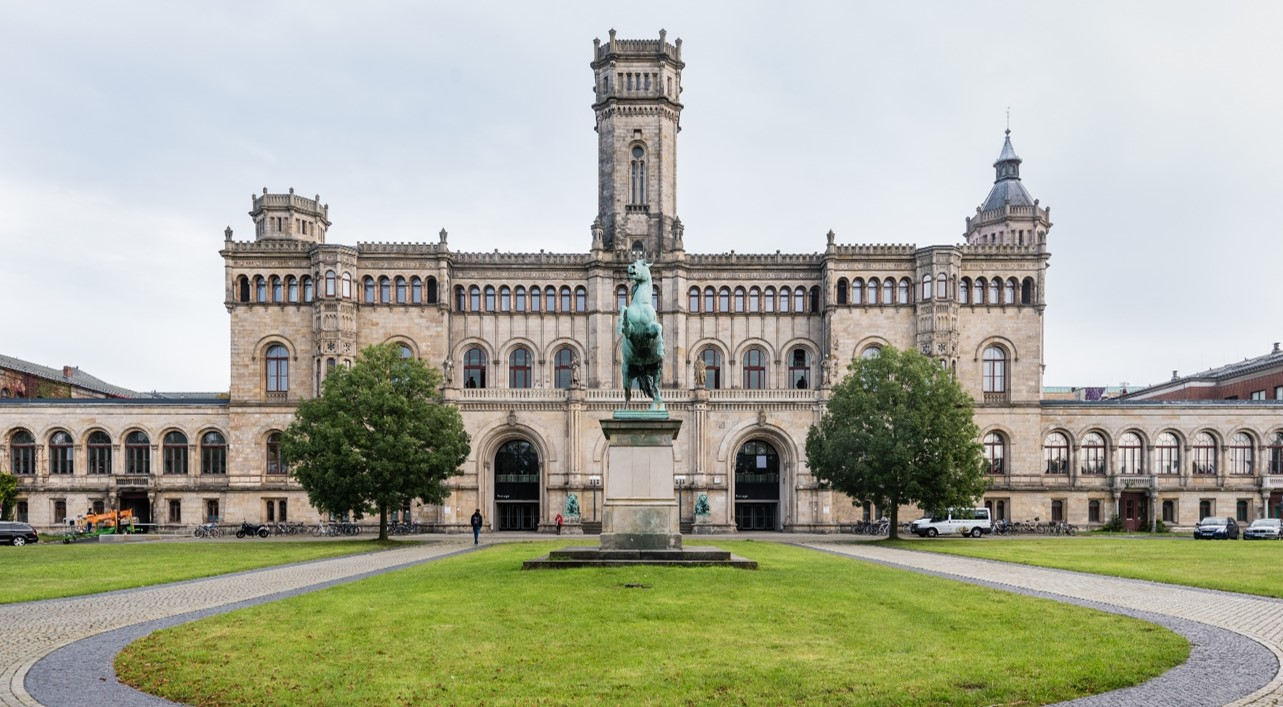
\includegraphics[width=0.75\textwidth]{figures/luh_default_presentation_title_image.jpg}}

\author[Abedjan \& Lindauer]{Ziawasch Abedjan \& Marius Lindauer\\[1em]
	
\includegraphics[height=\logoheight]{../latex_main/figures/luh_logo_rgb_0_80_155.pdf}\qquad
	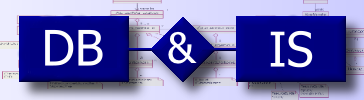
\includegraphics[height=\logoheight]{../latex_main/figures/DBIS_Kurzlogo.png}\qquad

\includegraphics[height=\logoheight]{../latex_main/figures/TNT_darkv4}\qquad

\includegraphics[height=\logoheight]{../latex_main/figures/L3S.jpg}	}
\date{Summer Term 2022; \hspace{0.5em} {
\includegraphics[height=1.5em]{../latex_main/figures/Cc-by-nc-sa_icon.svg.png}}; based on \href{https://ds100.org/fa21/}{[DS100]}
}


%%% Custom Packages
%----------------------------------------------------------------------
% Create dummy content
\usepackage{blindtext}

% Adds a frame with the current page layout. Just call \layout inside of a frame.
\usepackage{layout}


%%% Macros
%\renewcommand{\vec}[1]{\mathbf{#1}}
% \usepackage{bm}
%\let\vecb\bm

\title[Introduction]{DS: Introduction to Modeling}
\subtitle{Summary statistics and notation}

\graphicspath{ {./figure/} }
%\institute{}


\begin{document}
	
	\maketitle
	\begin{frame}{A simple model – the constant model}
	\begin{columns}
	  \begin{column}{.8\textwidth}
	    Suppose you want to build a model to predict some numerical quantity of a population:\\
	    \begin{itemize}
	        \item The percentage tip given at restaurants.
	        \item The weight of dogs.
	        \item The GPA of students at UC Berkeley.
	    \end{itemize}
	    One choice of model would be to ignore any relationships between variables, and predict the same number for each individual – i.e., predicting a constant. We call this a summary statistic because it summarizes the data in our sample.
	    \begin{itemize}
	        \item For instance, tips given at restaurants likely depend on the total bill price, the time of day, how generous the customers are feeling, et
	        \item Ignoring these factors is a simplifying assumption!
	    \end{itemize}
	  \end{column}
	  
	  
	  \begin{column}{.2\textwidth}
	          \\
	          \vspace{1cm}
	          
\includegraphics[scale=.5]{Bild17}
	  \end{column}
	\end{columns}
	\end{frame}
	
	
	
	\begin{frame}{Example – Tips dataset}
	\begin{columns}
	  \begin{column}{.6\textwidth}
	    \begin{itemize}
	        \item For instance, suppose a server collected data about the tips that they received over time while working at some restaurant. (A histogram w/KDE is shown to the right.)
	        \item We want to pick a constant that “best models” the tips we’ve seen. It seems like most tips are somewhere around 12-20\%.
	        \begin{itemize}
	            \item 15\% seems like a better guess than 25\%.
	            \item But is 15\% a better guess than 14\%? Hard to tell. 
	            \item We need a precise formulation of all of this.
	        \end{itemize}
	    \end{itemize}
	  \end{column}
	  
	  
	  \begin{column}{.4\textwidth}
	          \\
	          \vspace{1cm}
	          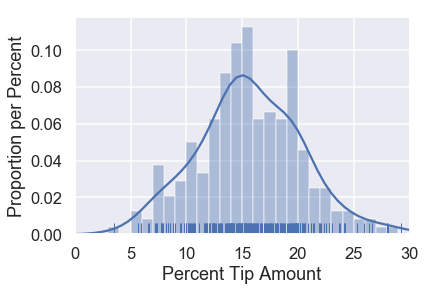
\includegraphics[scale=.5]{Bild18}
	  \end{column}
	\end{columns}
	\end{frame}
	
	
	\begin{frame}{Notation}
	    \begin{columns}
	        \begin{column}{.1\textwidth}
	                \\
	                %\vspace{-.5cm}
	                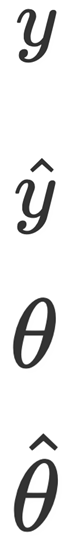
\includegraphics[scale=.43]{Bild19}
	        \end{column}
	        
	        
	        
	        \begin{column}{.9\textwidth}
	                represents our true observations (e.g. the actual observed tip \%s).\\
	                $y_i$ represents the ith observation in particular (e.g.   $y_4$  is the 4th observed tip). 
                    In general, we represent our collected data as    $y_1, y_2, \dots, y_n$               
                    \bigskip
                    represents the predicted observations given by our model (e.g. the predicted tip \%s).\\
                    $\hat{y_i}$ represents the ith prediction in particular (e.g.   $\hat{y_9}$     is the predicted tip for the 9th data point). 
                    
                    \bigskip
                    represents the parameter(s) of our model. This is what we are trying to estimate!\\
                    Parameters are what define our model. We make this more clear in the next slide.
                    
                    \vspace{.75cm}
                    represents the fitted, or optimal, parameter(s) that we solve for. It is our goal to find this!\\
                    We want to find   $\hat{\theta}$   to make the best possible model.

	        \end{column}
	    \end{columns}
	\end{frame}
	
	
	
	
	\begin{frame}{Notation}
	    The constant model can be stated as follows:\\ 
	    \hspace{7cm} $\hat{y} = \theta$
	    \begin{itemize}
	        \item Parameters are what define our model. Parameters tell us what the relationships between our input and output variables are.
	        \begin{itemize}
	            \item Note: not all models have parameters. KDEs are non-parametric models!
	        \end{itemize}
	        \item Our model only has one parameter. Here, the only thing that defines our model is the single number we will predict, regardless of the input.
	        \item Models can have many parameters (which we often express as a single parameter vector). Here are examples of models we’ll see in the coming lectures:
	        \begin{align*}
	            \hat{y} = \theta_0 + \theta_1 x \hspace{2cm} \hat{y} = \frac{1}{1+ exp(-x^T\Vec{\theta})}
	        \end{align*}
	        \item Our goal is to find the best possible value of our parameter, which we denote with  \hat{\theta}.
	        \begin{itemize}
	            \item We know that   $\hat{\theta}$    for the tips dataset is closer to 15\% than it is to 25\%.
	        \end{itemize}
	    \end{itemize}
	\end{frame}
	
	
	\begin{frame}{Prediction vs. estimation}
	    These terms are often used somewhat interchangeably, but there is a subtle difference between them.\\
	    \bigskip
	    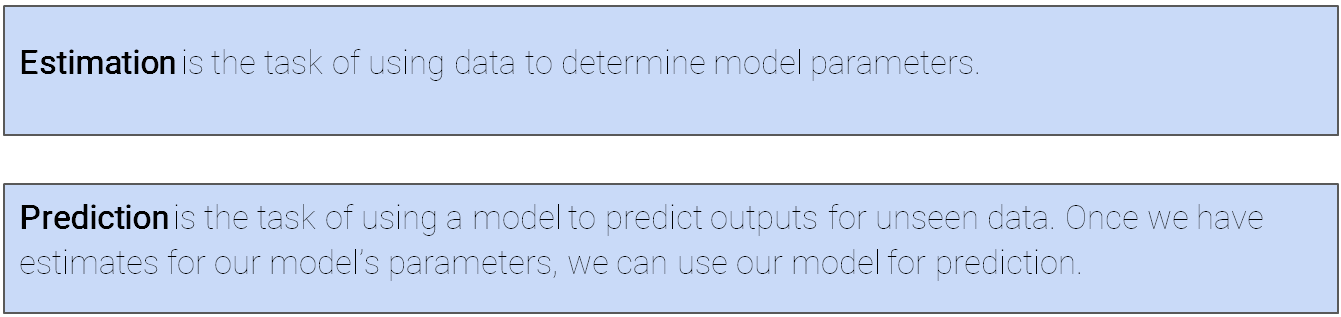
\includegraphics[scale=.4]{Bild20}
	\end{frame}
\end{document}